\subsection{Intel Lab Data}
\label{sec:intel-lab-data-evaluation}

We also evaluated our outlier detection framework on sensor data from the publicly available Intel Lab Data set~\footnote{\url{http://db.csail.mit.edu/labdata/labdata.html}}. The Intel Lab Data contains data collected from 54 sensors spread throughout the Intel Berkeley Research Lab. Each data entry contains information including humidity, temperature, light and voltage taken from a Micro2dot sensor and weatherboard. The dataset contains a total of approximately 2.3 million measurements.

The Intel lab dataset has known outliers from faulty sensor readings due to periods of critically low voltage. During these periods, the sensors go haywire and produce faulty measurements.

Due to the numerical nature of this data, the Simple Gaussian and Mixture models are well suited to analyzing it. However, the Histogram model does not fare as well.

% Random Sample 1000 data points
We analyzed a sample of 1000 data points selected at random from the data set. Figure~\ref{fig:sensors_1k_gm} shows the results from the simple Gaussian model comparing voltage and temperature; we set the tolerance ($\epsilon$) to 2. Since this model does not use correlation hints, the threshold for the statistical analyzer is irrelevant.

We observed that while this simple model is able to detect the high and low voltage outliers, it also identifies points within the main cluster of the data between 20 and 30 Celsius. These outliers are primarily due to light measurements whose measurements fall more than 2 standard deviations above the norm. When only outliers from temperature and voltage are taken into account, the outliers fall on the highest and lowest temperatures, as expected.

Figure~\ref{fig:sensors_1k_mm} shows the Mixture model results for the same 1000 randomly-selected data points. We used $0.75$ as the threshold $\theta$ to determine correlation, 3 Gaussians to populate our model, and returned $17\%$ of the data as outliers.

The statistical analyzer produces two correlations: one between temperature and voltage with an $R$ coefficient of $-0.75$ and between temperature and humidity with an $R$ of $-0.8$. The resulting Mixture models flags outliers that register temperatures of over 120 degrees. The outliers detected in the main cluster are the result of points that do not follow from the correlation between temperature and humidity.

\begin{figure}[h]
\centering
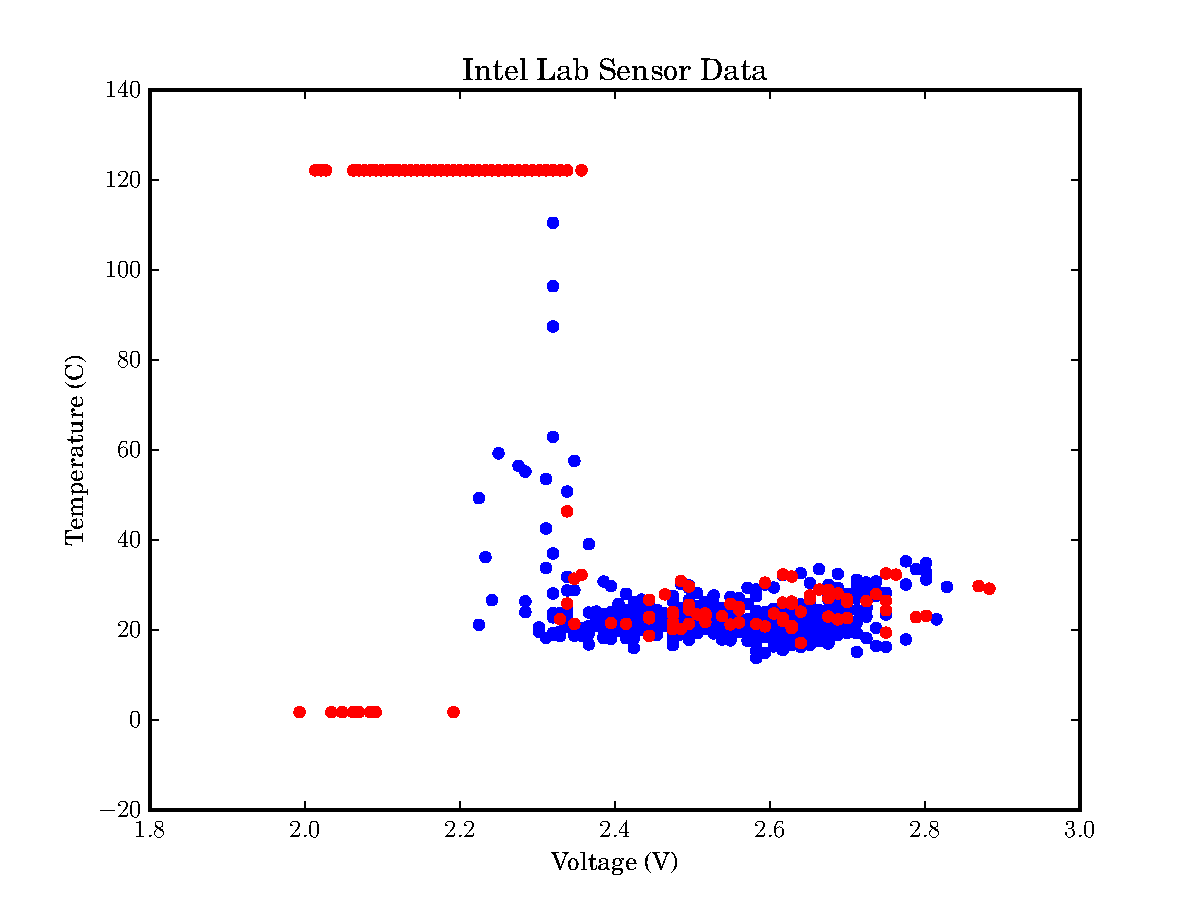
\includegraphics[width=0.45\textwidth]{../graphics/sensors_gm.pdf}
\caption{Outliers from sensor data detected by a Gaussian model.}
\label{fig:sensors_1k_gm}
\end{figure}
\begin{figure}[h]
\centering
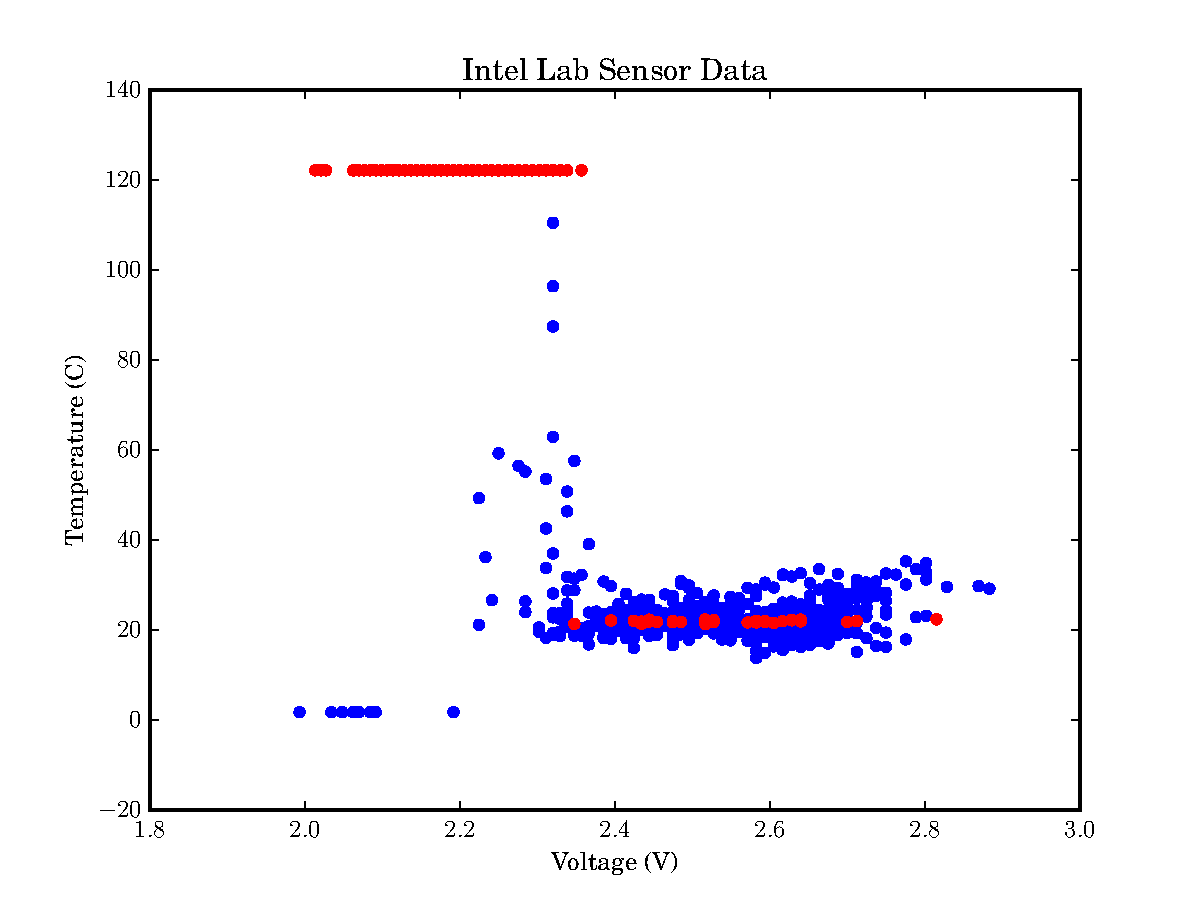
\includegraphics[width=0.45\textwidth]{../graphics/sensors_mm.pdf}
\caption{Outliers from sensor data detected by a Mixture model.}
\label{fig:sensors_1k_mm}
\end{figure}
